\chapter{Analisis}
Pada bab ini akan dipaparkan analisis yang dilakukan dalam pembuatan aplikasi
ini. Bagaimana data XML didapatkan dari situs \url{www.openstreetmap.org}
yang akan dibahas pada subbab \ref{ssec:analisis_osm} dan membacanya
menggunakan beberapa fungsi javascript yang akan dibahas
pada subbab \ref{ssec:analisis_js}. Setelah itu, data tersebut disimpan atau
dikonversi ke dalam bentuk graf sehingga dapat diimplementasikan algoritma
dijkstra untuk mencari rute terpendek dari satu node ke node lain. Berdasarkan 
informasi yang telah diolah, maka dapat dibuat visualisasi data atau informasi
tersebut menggunakan Google Maps Javascript API. Pada akhir bab ini, juga akan 
dibahas mengenai diagram \textit{use case} dan skenario untuk
memperjelas apa saja yang dapat dilakukan oleh \textit{user} pada aplikasi ini.

\section{Analisis OpenStreetMap} \label{ssec:analisis_osm}
OpenStreetMap adalah portal peta terbuka yang menyediakan data dalam bentuk peta
ataupun dokumen XML. Aplikasi yang dibuat akan berbasis OpenStreetMap, hal ini
berarti aplikasi yang dibuat akan menggunakan data yang diperoleh dari situs
\url{www.openstreetmap.org}. Untuk mendapatkan data peta pada situs
OpenStreetMap, user harus mengunjungi situs tersebut dan menggunakan fitur
\textit{export}. Data yang digunakan adalah data peta yang berbentuk
dokumen XML atau biasa disebut dengan OSMXML. Selanjutnya, informasi yang
terkandung di dalam dokumen OSMXML tersebut akan diproses untuk mengetahui node dan edge
pada peta. Informasi tersebut akan diubah ke dalam bentuk graf yang akan
diproses lebih lanjut menggunakan algoritma dijkstra untuk mengetahui jarak
terpendek dari satu node ke node lain.

\subsection{Langkah-Langkah Pengambilan Data OSMXML}
Berikut ini adalah langkah-langkah pengambilan data OSMXML yang akan digunakan:
\begin{enumerate}
  \item Mengunjungi situs \url{www.openstreetmap.org}.
  
  \item Menggunakan fitur \textit{search} untuk mencari area lokasi yang
  diinginkan. penggunaan fitur ini dapat dilihat pada Gambar
  \ref{fig:osmsearch_analisis} .
\begin{figure}[h]
\centering
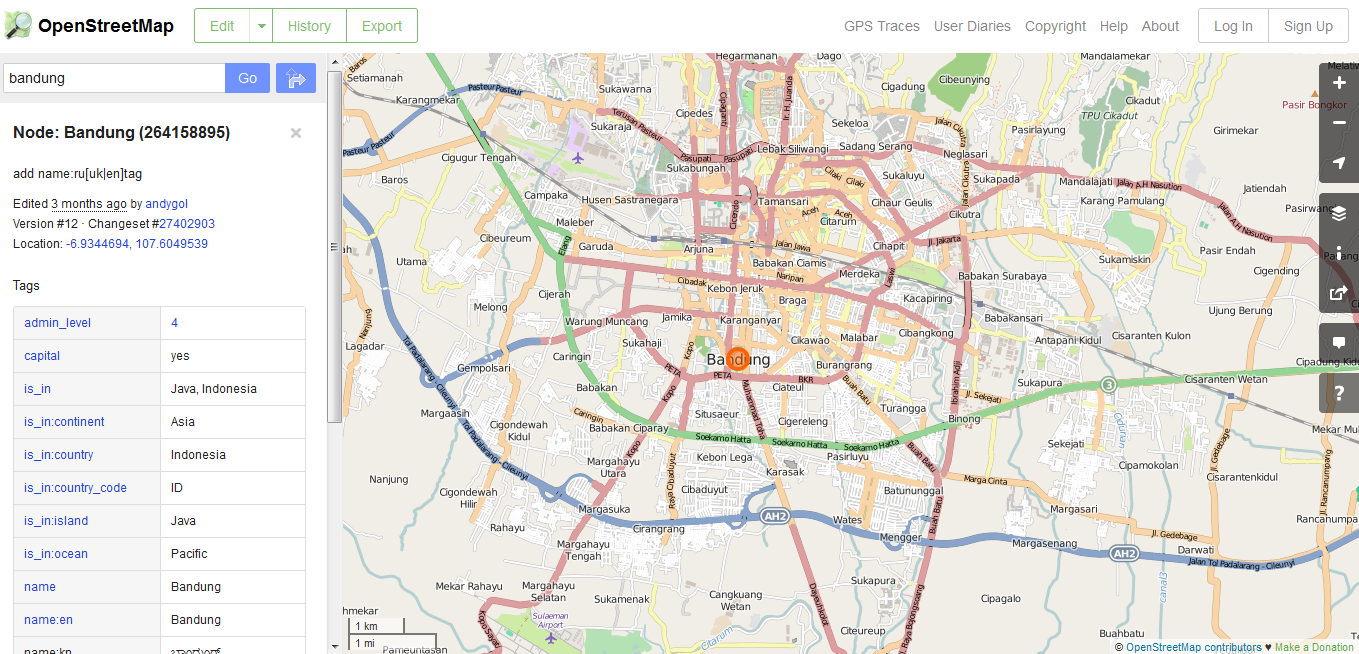
\includegraphics[scale=0.4]{Gambar/osmsearch_analisis}
\caption[Fitur search pada situs OpenStreetMap]{Fitur search pada situs
OpenStreetMap}
\label{fig:osmsearch_analisis}
\end{figure}
  
  \item Menggunakan fitur \textit{export} untuk mengunduh data dalam
  bentuk dokumen OSMXML. penggunaan fitur ini dapat dilihat pada Gambar
  \ref{fig:osmxml_analisis}.
\begin{figure}[h]
\centering
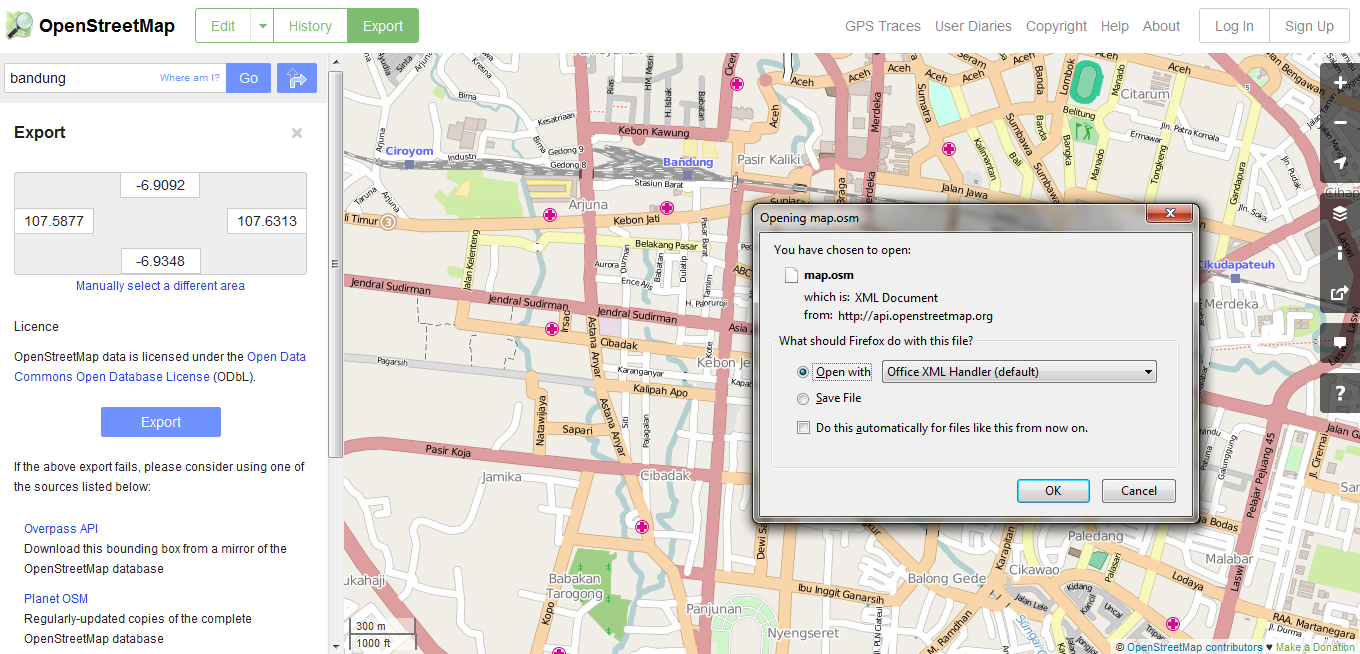
\includegraphics[scale=0.4]{Gambar/osmxml_analisis}
\caption[Fitur search pada situs OpenStreetMap]{Fitur \textit{export} pada situs
OpenStreetMap}
\label{fig:osmxml_analisis}
\end{figure}
\end{enumerate}

\subsection{OSMXML}
Sesuai dengan pembahasan pada subbab \ref{ssec:osmxml}, OSMXML merupakan dokumen
XML yang mengandung data-data peta OpenStreetMap. Berikut ini adalah dokumen
OSMXML yang sudah diunduh dan digunakan pada proses analisis.
\begin{lstlisting}
<?xml version="1.0" encoding="UTF-8"?>
<osm version="0.6" generator="CGImap 0.3.3 (29805 thorn-03.openstreetmap.org)" copyright="OpenStreetMap and contributors" attribution="http://www.openstreetmap.org/copyright" license="http://opendatacommons.org/licenses/odbl/1-0/">
 <bounds minlat="-6.9076500" minlon="107.5961800" maxlat="-6.9044500" maxlon="107.6016300"/>
 <node id="25418868" visible="true" version="6" changeset="27915808" timestamp="2015-01-04T17:54:58Z" user="isonpurba" uid="2552445" lat="-6.9064389" lon="107.5976351"/>
 <node id="25433683" visible="true" version="3" changeset="839915" timestamp="2009-03-21T14:18:48Z" user="adhitya" uid="7748" lat="-6.9067659" lon="107.5989458"/>
 ...
 <node id="25433687" visible="true" version="2" changeset="839915" timestamp="2009-03-21T14:18:36Z" user="adhitya" uid="7748" lat="-6.9040267" lon="107.5969508"/>
 <node id="25433688" visible="true" version="2" changeset="839915" timestamp="2009-03-21T14:18:58Z" user="adhitya" uid="7748" lat="-6.9039393" lon="107.5963723"/>
 <node id="25500626" visible="true" version="3" changeset="839915" timestamp="2009-03-21T14:22:17Z" user="adhitya" uid="7748" lat="-6.9070329" lon="107.6019401"/>
 ...
<node id="3030289971" visible="true" version="1" changeset="24892866" timestamp="2014-08-20T18:40:31Z" user="albahrimaraxsa" uid="2162153" lat="-6.9066710" lon="107.5982569"/>
 <node id="2325451442" visible="true" version="4" changeset="27916144" timestamp="2015-01-04T18:06:33Z" user="isonpurba" uid="2552445" lat="-6.9045011" lon="107.6024922"/>
 <way id="4567626" visible="true" version="4" changeset="15861148" timestamp="2013-04-25T13:56:12Z" user="mrdoggie94" uid="1331966">
  <nd ref="25433682"/>
  <nd ref="25433681"/>
  <nd ref="25433680"/>
  <tag k="avgspeed" v="15"/>
  <tag k="highway" v="residential"/>
  <tag k="name" v="Dr. Rubini"/>
 </way>
 <way id="4567634" visible="true" version="2" changeset="7821743" timestamp="2011-04-10T11:15:30Z" user="evo2mind" uid="234610">
  <nd ref="25433681"/>
  <nd ref="28802396"/>
  <tag k="avgspeed" v="15"/>
  <tag k="highway" v="residential"/>
  <tag k="name" v="Dr. Susilo"/>
 </way>
 ...
</osm>
\end{lstlisting}
Node dan way memiliki informasi penting yang akan digunakan pada aplikasi. Pada
tag node terdapat atribut id yang menunjukkan id pada setiap node, kemudian
terdapat atribut lat dan lon yang memberikan informasi titik koordinat
(\textit{latitude} dan \textit{longitude})pada node tersebut. Informasi yang
didapatkan akan disimpan ke dalam bentuk node pada graf. Tag way akan
menunjukkan hubungan pada node-node yang terdapat pada dokumen, dan akan
disimpan sebagai edge pada graf. Selain itu, tag way tidak hanya memberikan
informasi jalan raya atau jalan besar saja, tetapi juga beberapa elemen peta
lain seperti area sekeliling bangunan atau area sekitar tempat parkir. Maka dari
itu, diperlukan \textit{filter} pada tag way, karena hanya informasi jalan raya
atau jalan besar saja yang diperlukan oleh aplikasi. Data atau dokumen OSMXML
yang telah diperoleh, selanjutnya akan dibaca menggunakan javascript yang akan
dibahas pada subbab \ref{ssec:analisis_js}.

\section{Analisis Javascript} \label{ssec:analisis_js}
Javascript diperlukan untuk membaca dokumen OSMXML, sehingga seluruh informasi
yang diperlukan dapat diubah ke dalam bentuk graf yang akan diproses lebih lanjut.
XMLHttpRequest adalah salah satu objek pada javascript yang dapat digunakan 
untuk mendapatkan \textit{file} XML. Berikut ini adalah langkah-langkah yang
dilakukan untuk membaca dokumen OSMXML menggunakan javascript:
\begin{enumerate}
  \item Membuat Objek XMLHttpRequest. 
\begin{verbatim}
xmlhttp=new XMLHttpRequest();
xmlhttp.open("GET","map.xml",false);
xmlhttp.send();
xmlDoc=xmlhttp.responseXML;
\end{verbatim}
Objek XMLHttpRequest digunakan untuk membaca \textit{file} XML yang telah
diunduh sebelumnya. Tahap-tahap yang dilakukan adalah sebagai berikut:
\begin{enumerate}
  \item Membuat objek XMLHttpRequest.
  
  \item Objek ini akan menginisialisasi permintaan dengan memanggil fungsi
  open(), pada kode program di atas menggunakan \textit{method} ``GET'' yaitu meminta dokumen ``map.xml'' 
  dan parameter ``false'' menunjukkan bahwa permintaan tersebut \textit{synchronous}.
  
  \item Objek mengirimkan permintaan yang telah diinisialisasi sebelumnya dengan
  memanggil \textit{method} send();
  
  \item Tahap terakhir adalah mendapatkan respon dari permintaan yang telah
  dikirimkan. Objek mengakses atribut responseXML, jika permintaan berhasil
  maka variabel xmlDoc akan berisi dokumen XML yang diminta, jika gagal maka
  variabel akan bernilai \textit{null}.
\end{enumerate}

  \item Menampilkan informasi node yang didapat pada layar.
\begin{verbatim}
document.write("<div style='float: left'>");
document.write("<table><tr><th>Node</th><th>Id</th>
<th>Latitude</th><th>Longitude</th></tr>");
document.write("<caption>Node</caption>");

var node=xmlDoc.getElementsByTagName("node");
for (i=0;i<node.length;i++){
  document.write("<tr><td>");
  document.write(i);
  document.write("</td><td>");
  document.write(node[i].getAttribute('id'));
  document.write("</td><td>");
  document.write(node[i].getAttribute('lat'));
  document.write("</td><td>");
  document.write(node[i].getAttribute('lon'));
  document.write("</td></tr>");
}
document.write("</table>");
document.write("</div>");
\end{verbatim}
Kode diatas menampilkan informasi node pada dokumen OSMXML dalam bentuk tabel.
Berikut ini adalah tahap-tahap yang dilakukan:
\begin{enumerate}
  \item Membuat tag <div> sebagai tempat tabel.
  
  \item Membuat tabel.
  
  \item Membuat variabel node, variabel ini berisi informasi seluruh node yang
  terdapat pada variabel xmlDoc, \textit{method} yang digunakan adalah
  getElementsByTagName(). Sebelumnya xmlDoc sudah berisi dengan dokumen ``map.xml''.
  
  \item Melakukan \textit{print} pada tabel, beberapa atribut yang ditampilkan
  adalah id node, \textit{latitude}, dan \textit{longitude}.
\end{enumerate}

  \item Membuat fungsi untuk melakukan \textit{filter} pada elemen way.
\begin{verbatim}
function isHighway(way,index){
  var tag = way[index].getElementsByTagName("tag");
  for (hg=0;hg<tag.length;hg++){
    if(tag[hg].getAttribute('k') == "highway"){
      return true;
    }
  }
  return false;
}
\end{verbatim}
\textit{Filter} dilakukan karena hanya elemen way yang berjenis \textit{highway}
saja yang akan digunakan. Berikut ini adalah tahap-tahap yang dilakukan:
\begin{enumerate}
  \item Membuat fungsi isHighway() dengan parameter \textit{input} way dan
  index. Parameter way berisi informasi seluruh way, sedangkan parameter index
  menunjukkan tag way pada index tersebut yang akan dicari.
  
  \item Membuat variabel yang menyimpan informasi way pada index yang dicari,
  pada kode program variabel tersebut diberi nama ``tag''.
  
  \item Lakukan pengulangan untuk mencari setiap \textit{child} pada variabel
  ``tag'' yang memiliki atribut ``k=highway'', jika ditemukan fungsi akan
  mengembalikan \textit{true} dan \textit{false} jika tidak ditemukan.
\end{enumerate}
	
	\item Menampilkan informasi way yang didapat pada layar.
\begin{verbatim}
document.write("<div style='margin-left: 20px;float: left'>");
document.write("<table><tr><th>Way</th><th>Id Way</th>
<th>Edge</th><th>Id Node 1</th><th>Id Node 2</th></tr>");
document.write("<caption>Edge</caption>");

var way = xmlDoc.getElementsByTagName("way");
var nd;
for (i=0;i<way.length;i++){
  nd = way[i].getElementsByTagName("nd");
  if(isHighway(way,i)){
    for (j=0;j<nd.length-1;j++){
      document.write("<tr><td>");
      document.write(i);
      document.write("</td><td>");
      document.write(way[i].getAttribute('id'));
      document.write("</td><td>");
      document.write(j);
      document.write("</td><td>");
      document.write(nd[j].getAttribute('ref'));
      document.write("</td><td>");
      document.write(nd[j+1].getAttribute('ref'));	
      document.write("</td></tr>");
    }
  }
}
document.write("</div>");
\end{verbatim}
Kode diatas menampilkan informasi way pada dokumen OSMXML dalam bentuk tabel.
\begin{enumerate}
  \item Membuat tag <div> sebagai tempat tabel.
  
  \item Membuat tabel.
  
  \item Membuat variabel way, variabel ini berisi informasi seluruh way yang
  terdapat pada variabel xmlDoc, \textit{method} yang digunakan adalah
  getElementsByTagName(). Sebelumnya xmlDoc sudah berisi dengan dokumen ``map.xml''.
  
  \item Membuat variabel yang berisi informasi way pada index tertentu, dan
  lakukan \textit{filter} dengan menggunakan fungsi isHighway().
  
  \item Melakukan \textit{print} pada tabel, beberapa atribut yang ditampilkan
  adalah id way, id node pertama, dan id node kedua.
\end{enumerate}
\end{enumerate}
\begin{figure}[h]
\centering
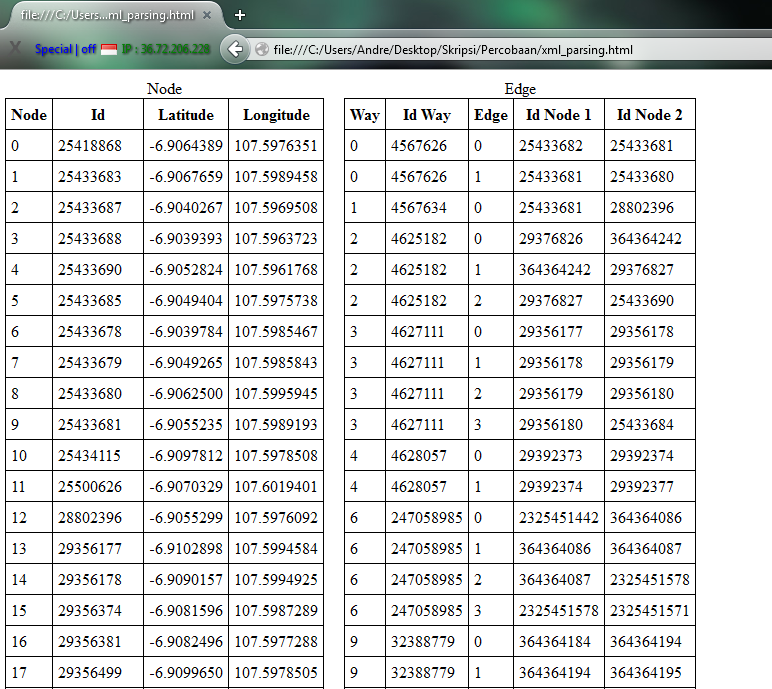
\includegraphics[scale=0.5]{Gambar/xml_parsing}
\caption[Parsing XML menggunakan Javascript]{Parsing XML menggunakan
Javascript}
\label{fig:xml_parsing}
\end{figure}
Hasil dari kode program di atas dapat dilihat pada Gambar \ref{fig:xml_parsing}.
Pada Gambar \ref{fig:xml_parsing} dapat dilihat terdiri dari dua tabel yang menunjukkan 
informasi node dan edge yang sudah dibaca. Tabel 
node menunjukkan atribut penting yang akan digunakan yaitu id node, \textit{latitude}, dan
\textit{longitude}. Sedangkan tabel edge menujukkan informasi yang didapatkan
dari tag way yang sudah dilakukan \textit{filter}, yaitu hanya tag way yang
memiliki \textit{child} highway saja yang akan digunakan. Pada tabel edge
terdapat informasi penting yang akan digunakan, yaitu id way, id node pertama, 
dan id node kedua. Informasi yang sudah didapatkan, selanjutnya akan dimodelkan
ke dalam bentuk graf yang akan dibahas pada subbab \ref{ssec:analisis_graf}.

\section{Menghitung Jarak Antara Dua Titik}
Untuk menghitung jarak antara dua titik dapat menggunakan rumus haversine atau
dikenal dengan haversine \textit{formula}. Analisis rumus haversine dilakukan
dengan implementasi rumus tersebut dengan contoh kasus perhitungan
jarak antara koordinat Kota Bandung (-6.9167,107.6000) dan koordinat Kota
Jakarta (-6.1745,106.8227). Berikut ini adalah rumus haversine yang telah
diimplementasikan:
\begin{verbatim}
function getDistance(lat1,lon1,lat2,lon2){
  var R = 6371; 
  var dLat = deg2rad(lat2-lat1); 
  var dLon = deg2rad(lon2-lon1); 
  var a = 
    Math.sin(dLat/2) * Math.sin(dLat/2) +
    Math.cos(deg2rad(lat1)) * Math.cos(deg2rad(lat2)) * 
    Math.sin(dLon/2) * Math.sin(dLon/2); 
  var c = 2 * Math.atan2(Math.sqrt(a), Math.sqrt(1-a)); 
  var d = R * c; 
  return d;
}

function deg2rad(deg){
  return deg * (Math.PI/180);
}
\end{verbatim}
Hasil yang ditunjukkan dari rumus haversine adalah 119.09781542340916 km dapat
dilihat pada Gambar \ref{fig:analisis_haver}.

\begin{figure}[h]
\centering
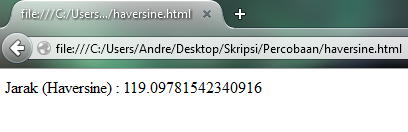
\includegraphics[scale=1]{Gambar/analisis_haver}
\caption[Perhitungan Jarak Dengan Haversine Formula]{Perhitungan Jarak Dengan Haversine Formula}
\label{fig:analisis_haver}
\end{figure}
Saat proses analisis, ternyata Google Maps Javascript API menyediakan suatu
\textit{library} untuk mengukur jarak antara dua titik. \textit{Library}
tersebut adalah \textit{geometry library} yang menyediakan fungsi utilitas yaitu
google.maps.geometry.spherical. Untuk menghitung jarak antara dua titik
digunakan fungsi computeDistanceBetween(). Sama seperti rumus haversine,
analisis fungsi computeDistanceBetween() dilakukan dengan implementasi contoh
kasus perhitungan jarak antara koordinat Kota Bandung dan Jakarta. Berikut ini
adalah fungsi computeDistanceBetween() yang telah diimplementasikan:
\begin{verbatim}
var jakarta = new google.maps.LatLng(-6.1745,106.8227);
var bandung = new google.maps.LatLng(-6.9167,107.6000);
var distance = google.maps.geometry.spherical.
computeDistanceBetween(jakarta, bandung);
\end{verbatim}
Hasil yang ditunjukkan dari fungsi computeDistanceBetween() adalah
119.23123264342443 km dapat dilihat pada Gambar \ref{fig:analisis_geometry}.

\begin{figure}[h]
\centering
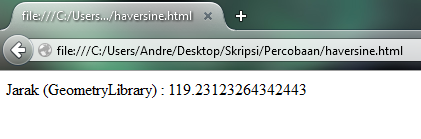
\includegraphics[scale=1]{Gambar/analisis_geometry}
\caption[Perhitungan Jarak Dengan Geometry Library]{Perhitungan Jarak Dengan
Geometry Library}
\label{fig:analisis_geometry}
\end{figure}
Terdapat perbedaan atau selisih yang dihasilkan oleh rumus haversine dan
fungsi computeDistanceBetween() sebesar 0.133417220015275 km. Fungsi 
computeDistanceBetween() yang akan digunakan untuk pembuatan aplikasi, bukan
rumus haversine. Hal ini karena fungsi tersebut lebih mudah digunakan.

\section{Pemodelan OSMXML Menjadi Graf} \label{ssec:analisis_graf}
Pada subbab \ref{ssec:analisis_js}, dokumen OSMXML sudah dibaca dan tahap
selanjutnya adalah memodelkan data OSMXML tersebut ke dalam bentuk graf. Seperti
yang sudah diketahui, graf terdiri dari node dan edge. Informasi node dan edge
yang sudah didapatkan akan dimodelkan ke dalam bentuk graf berarah, hal ini
karena jalan yang menghubungkan node-node tersebut memiliki arah, baik searah
maupun dua arah, arah jalan diketahui dengan melihat informasi tag oneway. Untuk
merepresentasikan graf tersebut akan digunakan \textit{adjacency list}.
Penggunaan \textit{adjacency list} disebabkan oleh penggunaan memori yang lebih
kecil dibandingkan dengan \textit{adjacency matrix}. Pada \textit{adjacency
list} memori yang digunakan adalah sebesar jumlah node yang terdapat pada
OSMXML, sedangkan pada \textit{adjacency matrix} memori yang digunakan adalah
nxn. Berikut ini adalah langkah-langkah yang dilakukan untuk memodelkan OSMXML
menjadi graf:
\begin{enumerate}
  \item Membuat kelas Node dan kelas Neighbor.
\begin{verbatim}
function Node(id, neighbors){
  this.id = id;
  this.adjList = neighbors;
}

function Neighbor(vnum, nbr, weight){
  this.vertexNum = vnum;
  this.weight = weight;
  this.next = nbr;
}
\end{verbatim}
Kedua kelas tersebut digunakan untuk menyimpan informasi id node dan jarak. Id
node disimpan pada kelas node menggunakan atribut id, sedangkan jarak disimpan
pada kelas neighbor menggunakan atribut weight.

  \item Membaca seluruh informasi node dan menyimpan pada kelas node.
\begin{verbatim}
var adjLists = [];
for(i=0;i<node.length;i++){
  adjLists.push(new Node(node[i].getAttribute('id'),null));
}
\end{verbatim}
  Berikut ini adalah tahap-tahap yang dilakukan untuk menyimpan seluruh
  informasi tersebut:
  \begin{enumerate}
    \item Membuat variabel adjLists, variabel ini bertipe array.
    
    \item Lakukan pengulangan untuk memasukkan informasi node satu persatu.
  \end{enumerate}

  \item Membuat fungsi untuk menentukan arah pada setiap node yang terhubung
  dengan node lain.
\begin{verbatim}
function wayDirection(way,index){
  var tag = way[index].getElementsByTagName("tag");
  for (hg=0;hg<tag.length;hg++){
    if(tag[hg].getAttribute('k') == "oneway"){
      return tag[hg].getAttribute('v');
    }
  }
  return false;
}
\end{verbatim}
  Berikut ini adalah tahap-tahap yang dilakukan:
  \begin{enumerate}
  \item Membuat fungsi wayDirection() dengan parameter \textit{input} way dan
  index. Parameter way berisi informasi seluruh way, sedangkan parameter index
  menunjukkan tag way pada index tersebut yang akan dicari informasi arahnya.
  
  \item Membuat variabel yang menyimpan informasi way pada index yang dicari,
  pada kode program variabel tersebut diberi nama ``tag''.
  
  \item Lakukan pengulangan untuk mencari setiap \textit{child} pada variabel
  ``tag'' untuk mencari atribut ``k=oneway'', jika ditemukan fungsi akan
  mengembalikan \textit{value} dari \textit{key} tersebut dan \textit{false}
  jika tidak ditemukan.
  \end{enumerate}

  \item Membuat fungsi untuk mendapatkan informasi koordinat node
  (\textit{latitude} dan \textit{longitude}).
\begin{verbatim}
function getLatByAtt(str){
  for (n=0;n<node.length;n++){
    if(node[n].getAttribute('id') == str){
      return node[n].getAttribute('lat');
    }
  }
  return -1;
}

function getLonByAtt(str){
  for (m=0;m<node.length;m++){
    if(node[m].getAttribute('id') == str){
      return node[m].getAttribute('lon');
    }
  }
  return -1;
}
\end{verbatim}
  Kode di atas terdiri dari dua fungsi, fungsi getLatByAtt() mencari informasi
  \textit{latitude} dan fungsi getLatByAtt() mencari informasi
  \textit{longitude}. Kedua fungsi tersebut melakukan pencarian node berdasarkan
  parameter \textit{input} str yang merupakan id node, jika ditemukan fungsi
  akan mengembalikan nilai \textit{latitude} atau \textit{longitude} dan
  mengembalikan nilai -1 jika tidak ditemukan.

  \item Membaca seluruh informasi edge yang terdapat pada tag way
\begin{verbatim}
for (i=0;i<way.length;i++){
  nd = way[i].getElementsByTagName("nd");
  if(isHighway(way,i)){
    oneway = wayDirection(way,i);
    for (j=0;j<nd.length-1;j++){
      //cari jarak 
      v1 = indexForId(adjLists,nd[j].getAttribute('ref'));
      v2 = indexForId(adjLists,nd[j+1].getAttribute('ref'));	
      lat1 = getLatByAtt(nd[j].getAttribute('ref'));
      lon1 = getLonByAtt(nd[j].getAttribute('ref'));
      lat2 = getLatByAtt(nd[j+1].getAttribute('ref'));
      lon2 = getLonByAtt(nd[j+1].getAttribute('ref'));
      
      point1 = new google.maps.LatLng(lat1,lon1);
      point2 = new google.maps.LatLng(lat2,lon2);
      distance = google.maps.geometry.spherical.
      computeDistanceBetween(point1,point2);
	  
      //memasukkan informasi edge		
      if(oneway == "yes"){
        adjLists[v1].adjList = new Neighbor(v2,
        adjLists[v1].adjList,distance); 
      }else if(oneway == "no"){
        adjLists[v1].adjList = new Neighbor(v2,
        adjLists[v1].adjList,distance); 
        adjLists[v2].adjList = new Neighbor(v1,
        adjLists[v2].adjList,distance);
      }else if(oneway == "-1"){
        adjLists[v2].adjList = new Neighbor(v1,
        adjLists[v2].adjList,distance); 
      }else{
        adjLists[v1].adjList = new Neighbor(v2,
        adjLists[v1].adjList,distance); 
        adjLists[v2].adjList = new Neighbor(v1,
        adjLists[v2].adjList,distance); 
      }	
    }
  }
}
\end{verbatim}
  Berikut ini adalah tahap-tahap yang dilakukan:
  \begin{enumerate}
    \item Melakukan pengulangan untuk setiap way.
    
    \item Melakukan \textit{filter} untuk setiap way, hanya ``highway'' saja
    yang akan dimasukkan informasinya ke dalam \textit{adjacency list}.
    
    \item Melakukan pemanggilan fungsi wayDirection() dan memasukkan nilai
    didapatkan dari fungsi tersebut ke variabel, pada kode di atas menggunakan
    variabel ``oneway''.
    
    \item Cari jarak antar node.
    
    \item Memasukkan informasi edge berdasarkan arah yang dimasukkan ke dalam
    variabel ``oneway''.
  \end{enumerate}

  \item Membuat fungsi untuk menampilkan graf ke layar
\begin{verbatim}
function print(list){
  for (j=0; j < list.length; j++){
    document.write(j);
    for (nbr=list[j].adjList; nbr != null;nbr=nbr.next) {
      document.write("---->");
      document.write('('+nbr.vertexNum+')');
    }
    document.write("<br>");
  }
}
\end{verbatim}
  Fungsi akan menerima parameter \textit{input} berupa array, yaitu
  variabel adjLists. Selanjutnya dilakukan pembacaan setiap index array dan
  hasilnya ditampilkan di layar.
\end{enumerate}
\begin{figure}[h]
\centering
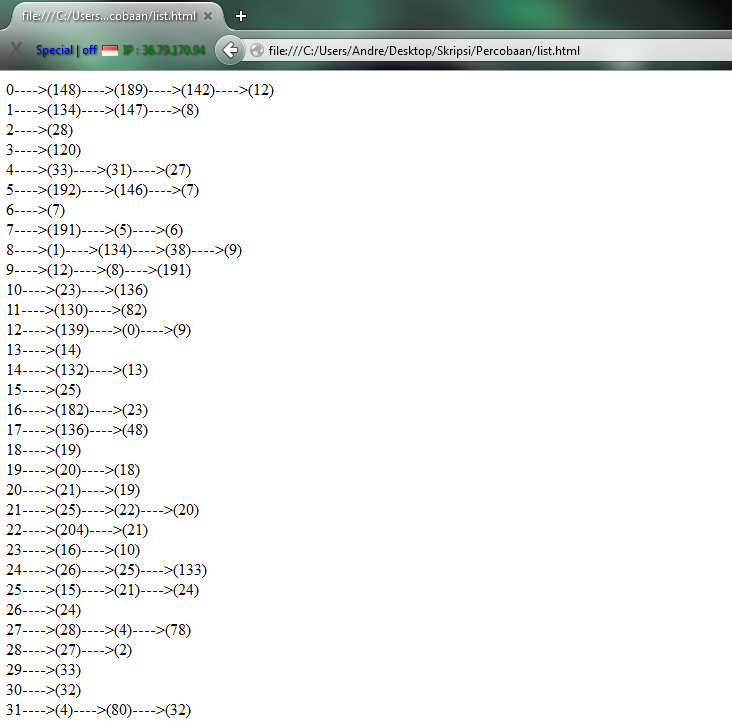
\includegraphics[scale=0.5]{Gambar/graf_analisis}
\caption[Pemodelan OSMXML menjadi Graf]{Pemodelan OSMXML menjadi Graf}
\label{fig:graf_analisis}
\end{figure}
Hasil dari kode program di atas dapat dilihat pada Gambar
\ref{fig:graf_analisis}.
Pada Gambar \ref{fig:graf_analisis}, data pada OSMXML sudah dimodelkan ke dalam
bentuk graf menggunakan representasi \textit{adjacency list}. Tahap selanjutnya
selanjutnya akan divisualisasikan menggunakan Google Maps Javascript API yang 
akan dibahas pada subbab \ref{ssec:analisis_gmap}.

\section{Visualisasi} \label{ssec:analisis_gmap}
Data OSMXML yang sudah dimodelkan ke dalam bentuk graf, selanjutnya akan
divisualisasikan menggunakan Google Maps Javascript API. Peta yang akan
ditampilkan dalam bentuk \textit{roadmap}, karena peta jenis ini memberikan 
informasi mengenai nama jalan, sehingga peta jenis ini lebih cocok untuk aplikasi 
yang akan dibangun. Berikut ini langkah-langkah yang dilakukan untuk membuat
visualisasi graf:
\begin{enumerate}
  \item Melakukan \textit{load} Google Maps Javascript API.
\begin{verbatim}
<script src="https://maps.googleapis.com/maps/api
/js?v=3.exp&libraries=geometry"></script>
\end{verbatim}

  \item Membuat elemen div sebagai wadah atau tempat untuk peta.
\begin{verbatim}
<div id="googleMap" style="width:75%;height:600px;float:left"></div>
\end{verbatim}
  
  \item Membuat objek google.maps.Map dengan parameter \textit{input map
  options} (variabel mapProp). Peta disisipkan pada elemen div yang memiliki id
  googleMap.
\begin{verbatim}
var mapProp = {
  center:new google.maps.LatLng(-6.906845432118958,107.59851515293121),
  zoom:17,
  mapTypeId:google.maps.MapTypeId.ROADMAP
};

var map=new google.maps.Map(document.getElementById("googleMap"),mapProp);
\end{verbatim}
  Berikut ini tahap-tahap yang dilakukan:
  \begin{enumerate}
    \item Membuat variabel untuk mendefinisikan properti peta, pada kode
    di atas dilakukan pengaturan titik tengah, zoom pada level 17, dan tipe peta
    yaitu ``ROADMAP''.
    
    \item Membuat objek google.maps.Map, objek tersebut memiliki parameter
    properti peta (variabel mapProp), selanjutnya peta disisipkan pada elemen
    div yang memiliki id googleMap.
  \end{enumerate}

  \item Membuat objek \textit{marker} untuk setiap node pada peta.
\begin{verbatim}
for (j=0;j<nd.length;j++){
  id = uniqueId();
  marker = new google.maps.Marker({
    id: id,
    position: new google.maps.LatLng(getLatByAtt(nd[j].getAttribute('ref')),
    getLonByAtt(nd[j].getAttribute('ref'))), map: map,
    icon: image,
  });
  markers[id] = marker;
\end{verbatim}
  Dilakukan pengulangan untuk setiap node dan membuat objek \textit{marker},
  membaca atribut \textit{latitude} dan \textit{longitude}, lalu menampilkan
  seluruh \textit{marker} pada peta.

  \item Membuat objek \textit{polyline} yang menghubungkan setiap node pada
  peta.
\begin{verbatim}
for (k=0;k<nd.length-1;k++){
  line = new google.maps.Polyline({
    path: [new google.maps.LatLng(getLatByAtt(nd[k].getAttribute('ref')),
    getLonByAtt(nd[k].getAttribute('ref'))), new
    google.maps.LatLng(getLatByAtt(nd[k+1].getAttribute('ref')),
    getLonByAtt(nd[k+1].getAttribute('ref')))], 
    strokeColor: "#000000",
    strokeOpacity: 1.0, 
    strokeWeight: 3,
    map: map
  });
}
\end{verbatim}
  
  \item Membuat fungsi untuk menambahkan \textit{info window} pada setiap node
  untuk memberikan informasi id dan index node.
\begin{verbatim}
function addInfoWindow(marker, message) {
  var infoWindow = new google.maps.InfoWindow({
    content: message
  });
  
  google.maps.event.addDomListener(marker, 'click', function () {
    infoWindow.open(map, marker);
  });
}
\end{verbatim}
  Berikut ini adalah tahap-tahap yang dilakukan:
  \begin{enumerate}
    \item Membuat fungsi addInfoWindow dengan parameter \textit{input} yaitu
    \textit{marker} dan pesan.
    
    \item Membuat objek google.maps.InfoWindow.
    
    \item Menambahkan objek google.maps.InfoWindow pada \textit{listener} yang
    berasosiasi dengan parameter \textit{marker}.
  \end{enumerate}
\end{enumerate}
\begin{figure}[h]
\centering
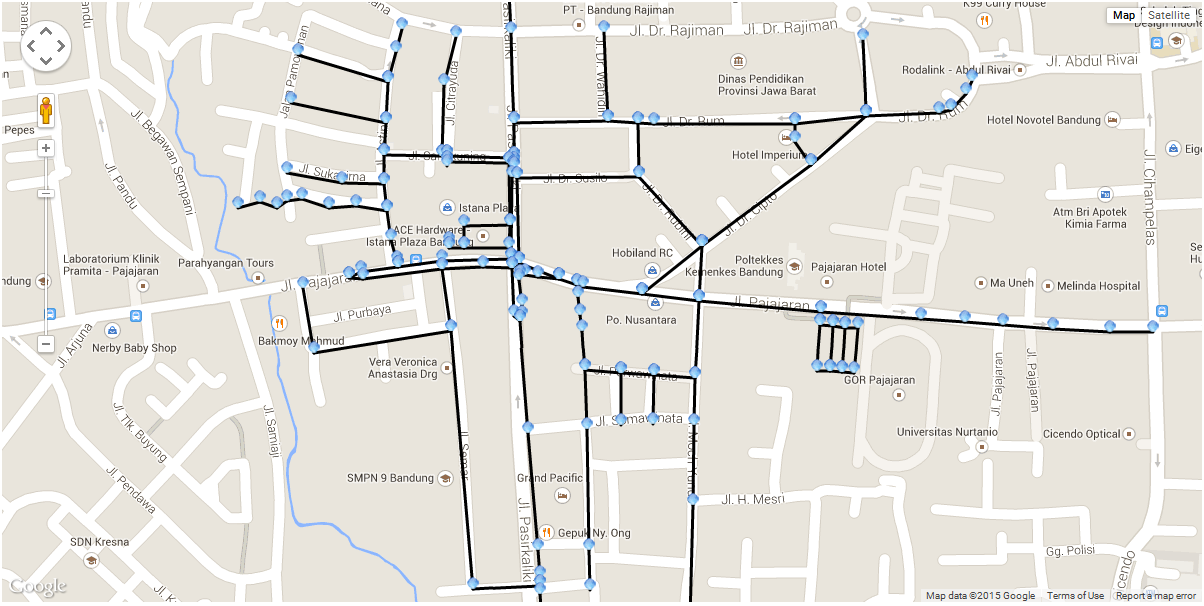
\includegraphics[scale=0.5]{Gambar/visualisasi_graf}
\caption[Visualisasi]{Visualisasi}
\label{fig:visualisasi}
\end{figure}
Hasil dari langkah-langkah di atas dapat dilihat pada Gambar
\ref{fig:visualisasi}. Setiap node pada graf yang sudah dilakukan
\textit{filter} akan diwakili oleh marker. Setiap marker tersebut akan memiliki \textit{info
window} yang akan memberikan informasi seperti id node, index node pada graf,
dan dua buah \textit{hyperlink} yang berfungsi untuk menjadikan marker yang
dipilih menjadi asal atau tujuan. Contoh \textit{info window} yang ditampilkan
pada peta dapat dilihat pada Gambar \ref{fig:visualisasi_infowindow}. Setiap
edge pada graf akan menjadi garis pada peta yang dibuat menggunakan \textit{polyline}.
\begin{figure}[h]
\centering
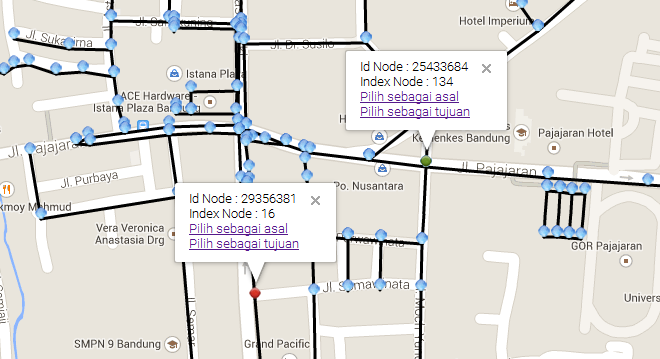
\includegraphics[scale=0.8]{Gambar/visualisasi_infowindow}
\caption[Info Window]{Info Window}
\label{fig:visualisasi_infowindow}
\end{figure}

\section{Algoritma Dijkstra}
Untuk pencarian rute terdekat, aplikasi menggunakan algoritma dijkstra.
Algoritma tersebut diimplementasikan pada graf yang sudah dimodelkan
sebelumnya. Berikut ini adalah langkah-langkah algoritma dijkstra yang
digunakan:
\begin{enumerate}
  \item Membuat kelas Dijkstra dan inisialisasi variabel.
\begin{verbatim}
function Dijkstra(){
  var INFINITY = 1/0;
  this.nodes = {};
}
\end{verbatim}

  \item Membuat fungsi untuk menambahkan node. 
\begin{verbatim}
this.addNode = function(name,edges){
  this.nodes[name] = edges;
}
\end{verbatim}

  \item Implementasi algoritma dijkstra
\begin{verbatim}
this.shortestPath = function(asal, tujuan){
  var PQ = new PriorityQueue();
  var distances = {};
  var previous = {};
  var path = [];
  var smallest, node, neighbor, alt;

  for(node in this.nodes){
    if(node === asal){
      distances[node] = 0;
      PQ.enqueue(0, node);
    }
    else{
      distances[node] = INFINITY;
      PQ.enqueue(INFINITY, node);
    }
    previous[node] = null;
  }

  while(!PQ.isEmpty()){
    smallest = PQ.dequeue();
    if(smallest === tujuan){
      while(previous[smallest]){
        path.push(smallest);
        smallest = previous[smallest];
      }
      break;
    }

    if(!smallest || distances[smallest] === INFINITY){
      continue;
    }

    for(neighbor in this.nodes[smallest]){
      alt = distances[smallest] + this.nodes[smallest][neighbor];
      if(alt < distances[neighbor]) {
        distances[neighbor] = alt;
        previous[neighbor] = smallest;
        PQ.enqueue(alt, neighbor);
      }
    }
  }
  return path;
}
\end{verbatim}
\end{enumerate}
Fungsi dijkstra akan menerima \textit{input} berupa objek ``edge'' yang berisi
informasi dari graf, selanjutnya fungsi akan mengeluarkan \textit{output}
yaitu jalur terpendek dari satu titik ke titik lain dalam bentuk array. Contoh
kasus yang digunakan, yaitu mencari rute terdekat dari titik asal ``16'' dan 
titik tujuan ``198'', output yang dihasilkan dapat dilihat pada Gambar
\ref{fig:output_dijkstra}.
\begin{figure}[h]
\centering
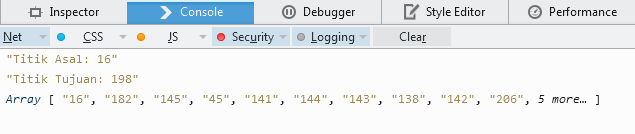
\includegraphics[scale=0.8]{Gambar/output_dijkstra}
\caption[Keluaran fungsi Dijkstra]{Keluaran fungsi Dijkstra}
\label{fig:output_dijkstra}
\end{figure}
Visualisasi rute terdekat dapat dilihat pada Gambar
\ref{fig:visualisasi_dijkstra}.
 \begin{figure}[h]
\centering
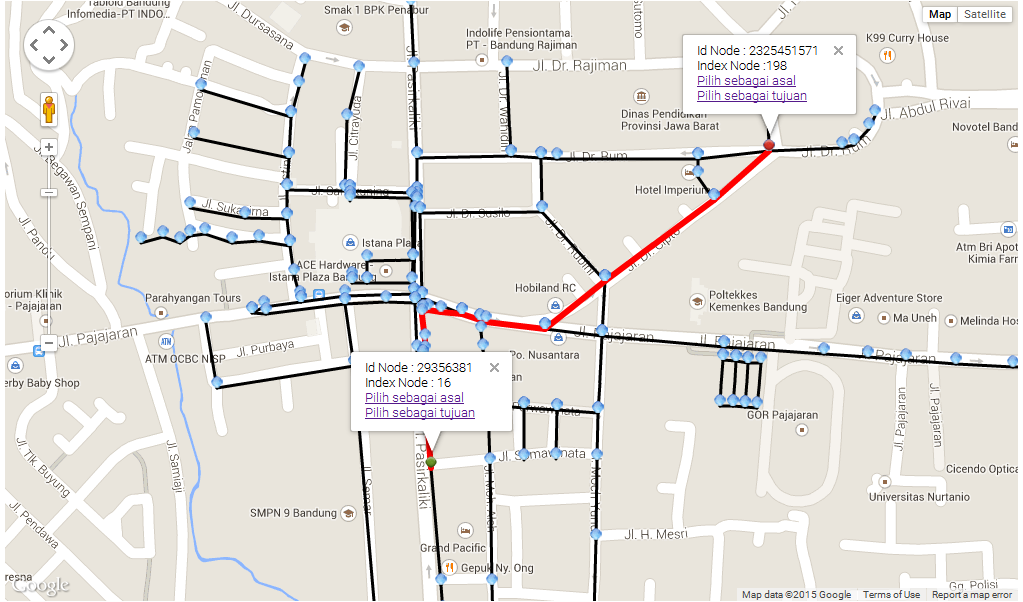
\includegraphics[scale=0.5]{Gambar/visualisasi_dijkstra}
\caption[Visualisasi Rute Terdekat]{Visualisasi Rute Terdekat}
\label{fig:visualisasi_dijkstra}
\end{figure}

\section{Analisis Berorientasi Objek}
Aplikasi pencarian rute terdekat yang dibangun akan mengolah data yang
disediakan oleh OpenStreetMap dalam bentuk XML dan memodelkannya ke dalam bentuk graf. 
\textit{User} dapat memilih titik asal dan titik tujuan, selanjutnya akan
diimplementasikan algoritma Dijkstra untuk mencari rute terdekat antara kedua titik 
tersebut dan menunjukkan hasilnya secara visual menggunakan Google Maps
Javascript API. Pada subbab ini akan membahas interaksi antara \textit{user}
dengan sistem yaitu menggunakan diagram \textit{use case} dan skenario. Setelahnya,
dibahas juga diagram kelas untuk menunjukkan kelas-kelas yang ada pada sistem
dan hubungannya.

\subsection{Diagram \textit{Use Case}}
Diagram \textit{use case} adalah pemodelan yang berfungsi memperjelas interaksi
antara aktor atau \textit{user} dengan sistem. 
Diagram \textit{use case} aplikasi pencarian rute terdekat dapat dilihat pada
Gambar \ref{fig:usecase}.
\begin{figure}[h]
\centering
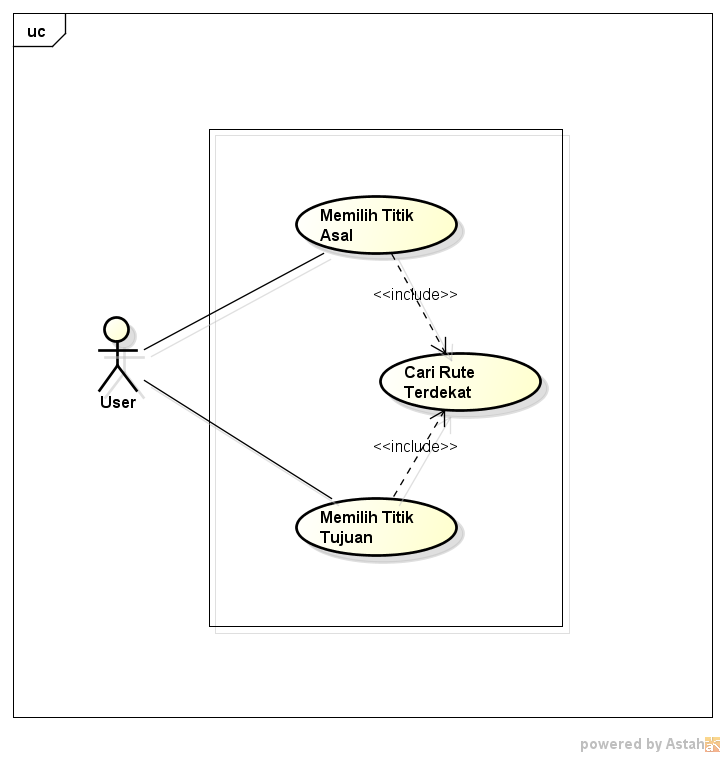
\includegraphics[scale=0.55]{Gambar/usecase}
\caption[Diagram Use Case]{Diagram \textit{use case}}
\label{fig:usecase}
\end{figure}

Berdasarkan analisis yang telah dilakukan, maka \textit{user} dapat melakukan
interaksi sebagai berikut:
\begin{enumerate}
  \item Memilih titik asal.\\
  \textit{User} dapat menekan salah satu \textit{marker} yang ada pada peta dan
  menekan \textit{link} ``pilih titik asal''. Selanjutnya, akan ditampilkan
  informasi titik yang sudah dipilih pada sisi kanan layar.
  
  \item Memilih titik tujuan.\\
  \textit{User} dapat menekan salah satu \textit{marker} yang ada pada peta dan
  menekan \textit{link} ``pilih titik tujuan''. Selanjutnya, akan ditampilkan
  informasi titik yang sudah dipilih pada sisi kanan layar.
  
  \item Mencari rute terdekat dari titik asal ke titik tujuan.\\
  \textit{User} dapat menekan tombol ``Cari'' untuk mencari rute terdekat dari
  kedua titik yang telah dipilih sebelumnya.
\end{enumerate}

\subsection{Skenario}
Berikut ini adalah skenario untuk setiap \textit{use case}:
\begin{enumerate}
  \item Skenario memilih titik asal dapat dilihat pada Tabel
  \ref{tab:titik_asal}.  
\begin{table}[h]
\centering
\caption{Skenario memilih titik asal} 
\label{tab:titik_asal}
\begin{tabular}{|c|c|}
\hline
Nama          & Memilih titik asal                                              \\ \hline
Aktor         & User                                                            \\ \hline
Kondisi Awal  & Titik asal belum terpilih                                       \\ \hline
Kondisi Akhir & Titik asal sudah terpilih dan ditampilkan di sisi kanan layar   \\ \hline
Skenario      & User menekan marker pada peta dan menekan link pilih titik asal \\ \hline
Deskripsi     & User memilih titik pada peta untuk dijadikan titik asal         \\ \hline
Eksepsi       & -                                                               \\ \hline
\end{tabular}
\end{table}

  \item Skenario memilih titik tujuan dapat dilihat pada Tabel
  \ref{tab:titik_tujuan}.
\begin{table}[h]
\centering
\caption{Skenario memilih titik tujuan} 
\label{tab:titik_tujuan}
\begin{tabular}{|c|c|}
\hline
Nama          & Memilih titik tujuan                                              \\ \hline
Aktor         & User                                                              \\ \hline
Kondisi Awal  & Titik tujuan belum terpilih                                       \\ \hline
Kondisi Akhir & Titik tujuan sudah terpilih dan ditampilkan di sisi kanan layar   \\ \hline
Skenario      & User menekan marker pada peta dan menekan link pilih titik tujuan \\ \hline
Deskripsi     & User memilih titik pada peta untuk dijadikan titik tujuan         \\ \hline
Eksepsi       & -                                                                 \\ \hline
\end{tabular}
\end{table}

  \item Skenario cari rute terdekat dapat dilihat pada Tabel
  \ref{tab:rute_terdekat}.
\begin{table}[h]
\centering
\caption{Skenario cari rute terdekat} 
\label{tab:rute_terdekat}
\begin{tabular}{|c|c|}
\hline
Nama          & Cari rute terdekat                                                                                        \\ \hline
Aktor         & User                                                                                                      \\ \hline
Kondisi Awal  & Titik asal dan titik tujuan sudah terpilih                                                                \\ \hline
Kondisi Akhir & Sistem menampilkan rute terdekat menggunakan polyline                                                     \\ \hline
Skenario      & User menekan tombol Cari!                                                                                 \\ \hline
Deskripsi     & \begin{tabular}[c]{@{}c@{}}User menekan tombol Cari! dan sistem menampilkan rute \\ terdekat\end{tabular}                        \\ \hline
Eksepsi       & \begin{tabular}[c]{@{}c@{}}Jika user belum memilih titik asal atau tujuan \\ akan ditampilkan alert atau peringatan\end{tabular} \\ \hline
\end{tabular}
\end{table}
\end{enumerate}

\subsection{Diagram Kelas Sederhana}
Pada bagian ini, akan dijelaskan diagram kelas yang digunakan untuk memenuhi
kebutuhan \textit{user} yang sudah dijelaskan pada bagian diagram \textit{use
case} dan skenario. Berikut ini adalah diagram kelas sederhana yang dapat
dilihat pada Gambar \ref{fig:diagram_kelas}.
\begin{figure}[h]
\centering
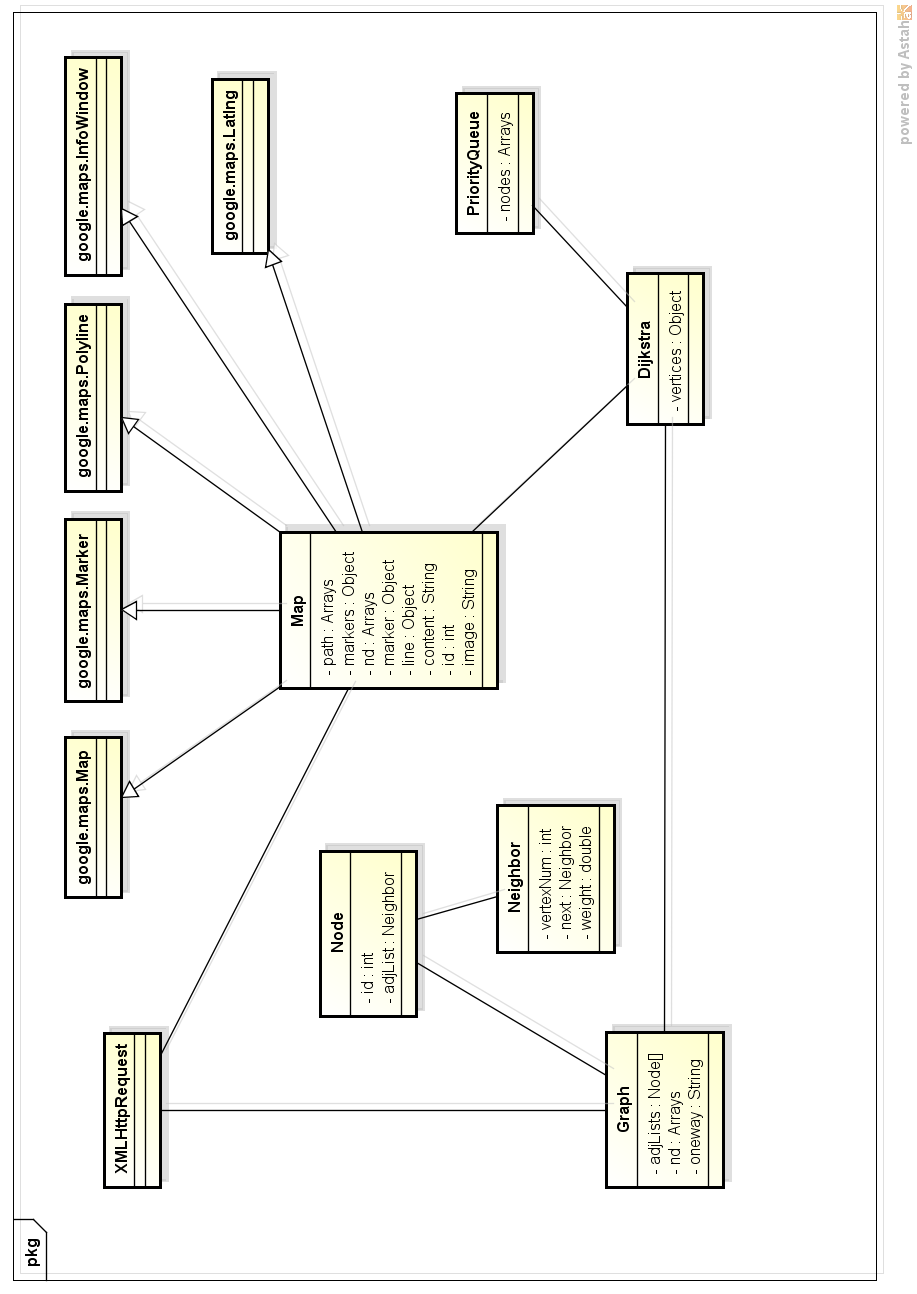
\includegraphics[scale=0.6]{Gambar/diagram_kelas}
\caption[Diagram Kelas Sederhana]{Diagram Kelas Sederhana}
\label{fig:diagram_kelas}
\end{figure}
Berikut ini adalah penjelasan dari setiap kelas yang terdapat pada diagram
kelas sederhana:
\begin{itemize}
  \item Kelas XMLHttpRequest\\
  Kelas ini berfungsi untuk melakukan \textit{load} dokumen OSMXML.
  
  \item Kelas Node dan Neighbor\\
  Kedua kelas ini akan menyimpan informasi yang didapatkan dari OSMXML sebagai
  representasi dari graf yaitu \textit{adjacency list}.
  
  \item Kelas Graph\\
  Kelas ini berfungsi untuk mengubah informasi yang didapatkan dari OSMXML
  menjadi graf.
  
  \item Kelas Map\\
  Kelas ini berfungsi untuk melakukan \textit{generate} peta, visualisasi graf,
  dan visualisasi rute terdekat.
  
  \item Kelas google.maps.Map\\
  Kelas ini berfungsi untuk membuat objek peta.
  
  \item Kelas google.maps.Marker\\
  Kelas ini berfungsi untuk membuat objek \textit{marker} yang akan digunakan
  sebagai visualisasi node pada peta.
  
  \item Kelas google.maps.Polyline\\
  Kelas ini berfungsi untuk membuat objek \textit{polyline} yang akan digunakan
  sebagai visualisasi edge pada peta.
  
  \item Kelas google.maps.InfoWindow\\
  Kelas ini berfungsi untuk membuat objek \textit{InfoWindow} yang akan
  disisipkan pada setiap objek \textit{marker}.
  
  \item Kelas google.maps.Latlng\\
  Kelas ini berfungsi untuk membuat objek Latlng. Latlng merupakan objek yang
  berisi informasi koordinat (\textit{latitude} dan \textit{longitude}).
  
  \item Kelas Dijkstra\\
  Kelas ini berfungsi untuk mencari rute terdekat berdasarkan \textit{input}
  titik asal dan titik tujuan.
  
  \item Kelas PriorityQueue\\
  Kelas ini merupakan struktur data \textit{queue} yang digunakan pada
  kelas dijkstra.
\end{itemize}



















